\chapter{Manipulação de bits}

Todos os dados em programas de computador são armazenados internamente como bits,
ou seja, como números 0 e 1.
Este capítulo discute a representação de bits
de inteiros e mostra exemplos
de como usar operações de bits.
Acontece que existem muitos usos para
manipulação de bits em programação de algoritmos.

\section{Representação de bits}

\index{representação de bits}

Na programação, um inteiro de $n$ bits é armazenado internamente
como um número binário que consiste em $n$ bits.
Por exemplo, o tipo \texttt{int} em C++ é
um tipo de 32 bits, o que significa que cada número \texttt{int}
consiste em 32 bits.

Aqui está a representação de bits do
número \texttt{int} 43:
\[00000000000000000000000000101011\]
Os bits na representação são indexados da direita para a esquerda.
Para converter uma representação de bits $b_k \cdots b_2 b_1 b_0$ em um número,
podemos usar a fórmula
\[b_k 2^k + \ldots + b_2 2^2 + b_1 2^1 + b_0 2^0.\]
Por exemplo,
\[1 \cdot 2^5 + 1 \cdot 2^3 + 1 \cdot 2^1 + 1 \cdot 2^0 = 43.\]

A representação de bits de um número é
\key{assinada} ou \key{não assinada}.
Geralmente uma representação assinada é usada,
o que significa que números negativos e positivos
podem ser representados.
Uma variável assinada de $n$ bits pode conter qualquer
inteiro entre $-2^{n-1}$ e $2^{n-1}-1$.
Por exemplo, o tipo \texttt{int} em C++ é
um tipo assinado, então uma variável \texttt{int} pode conter qualquer
inteiro entre $-2^{31}$ e $2^{31}-1$.

O primeiro bit em uma representação assinada
é o sinal do número (0 para números não negativos
e 1 para números negativos), e
os $n-1$ bits restantes contêm a magnitude do número.
\key{Complemento de dois} é usado, o que significa que o
número oposto de um número é calculado primeiro
invertendo todos os bits no número,
e depois aumentando o número por um.

Por exemplo, a representação de bits de
o número \texttt{int} $-43$ é
\[11111111111111111111111111010101.\]

Em uma representação não assinada, apenas os números não negativos
podem ser usados, mas o limite superior para os valores é maior.
Uma variável não assinada de $n$ bits pode conter qualquer
inteiro entre $0$ e $2^n-1$.
Por exemplo, em C++, uma variável \texttt{unsigned int}
pode conter qualquer inteiro entre $0$ e $2^{32}-1$.

Existe uma conexão entre as
representações:
um número assinado $-x$ é igual a um número não assinado $2^n-x$.
Por exemplo, o código a seguir mostra que
o número assinado $x=-43$ é igual ao número não assinado
$y=2^{32}-43$:
\begin{lstlisting}
int x = -43;
unsigned int y = x;
cout << x << "\n"; // -43
cout << y << "\n"; // 4294967253
\end{lstlisting}

Se um número for maior que o limite superior
da representação de bits, o número sofrerá overflow.
Em uma representação assinada,
o próximo número após $2^{n-1}-1$ é $-2^{n-1}$,
e em uma representação não assinada,
o próximo número após $2^n-1$ é $0$.
Por exemplo, considere o código a seguir:
\begin{lstlisting}
int x = 2147483647
cout << x << "\n"; // 2147483647
x++;
cout << x << "\n"; // -2147483648
\end{lstlisting}

Inicialmente, o valor de $x$ é $2^{31}-1$.
Este é o maior valor que pode ser armazenado
em uma variável \texttt{int},
então o próximo número após $2^{31}-1$ é $-2^{31}$.


\section{Operações de bits}

\newcommand\XOR{\mathbin{\char`\^}}

\subsubsection{Operação E}

\index{operação E}

A operação \key{E} $x$ \& $y$ produz um número
que tem bits iguais a um nas posições onde ambos
$x$ e $y$ têm bits iguais a um.
Por exemplo, $22$ \& $26$ = 18, porque

\begin{center}
\begin{tabular}{rrr}
& 10110 & (22)\\
\& & 11010 & (26) \\
\hline
 = & 10010 & (18) \\
\end{tabular}
\end{center}

Usando a operação E, podemos verificar se um número
$x$ é par porque
$x$ \& $1$ = 0 se $x$ é par, e
$x$ \& $1$ = 1 se $x$ é ímpar.
De forma mais geral, $x$ é divisível por $2^k$
exatamente quando $x$ \& $(2^k-1)$ = 0.

\subsubsection{Operação OU}

\index{operação OU}

A operação \key{OU} $x$ | $y$ produz um número
que tem bits iguais a um nas posições onde pelo menos um
de $x$ e $y$ tem bits iguais a um.
Por exemplo, $22$ | $26$ = 30, porque

\begin{center}
\begin{tabular}{rrr}
& 10110 & (22)\\
| & 11010 & (26) \\
\hline
 = & 11110 & (30) \\
\end{tabular}
\end{center}

\subsubsection{Operação XOR}

\index{operação XOR}

A operação \key{XOR} $x$ $\XOR$ $y$ produz um número
que tem bits iguais a um nas posições onde exatamente um
de $x$ e $y$ tem bits iguais a um.
Por exemplo, $22$ $\XOR$ $26$ = 12, porque

\begin{center}
\begin{tabular}{rrr}
& 10110 & (22)\\
$\XOR$ & 11010 & (26) \\
\hline
 = & 01100 & (12) \\
\end{tabular}
\end{center}

\subsubsection{Operação NÃO}

\index{operação NÃO}

A operação \key{NÃO} \textasciitilde$x$
produz um número onde todos os bits de $x$
foram invertidos.
A fórmula \textasciitilde$x = -x-1$ é válida,
por exemplo, \textasciitilde$29 = -30$.

O resultado da operação NÃO no nível de bits
depende do comprimento da representação de bits,
porque a operação inverte todos os bits.
Por exemplo, se os números são de 32 bits
números \texttt{int}, o resultado é o seguinte:

\begin{center}
\begin{tabular}{rrrr}
$x$ & = & 29 &   00000000000000000000000000011101 \\
\textasciitilde$x$ & = & $-30$ & 11111111111111111111111111100010 \\
\end{tabular}
\end{center}

\subsubsection{Deslocamentos de bits}

\index{deslocamento de bits}

O deslocamento de bits para a esquerda $x < < k$ anexa $k$
bits zero ao número,
e o deslocamento de bits para a direita $x > > k$
remove os $k$ últimos bits do número.
Por exemplo, $14 < < 2 = 56$,
porque 14 e 56 correspondem a 1110 e 111000.
Da mesma forma, $49 > > 3 = 6$,
porque 49 e 6 correspondem a 110001 e 110.

Observe que $x < < k$
corresponde a multiplicar $x$ por $2^k$,
e $x > > k$
corresponde a dividir $x$ por $2^k$
arredondado para baixo para um inteiro.

\subsubsection{Aplicações}

Um número da forma $1 < < k$ tem um bit
na posição $k$ e todos os outros bits são zero,
então podemos usar esses números para acessar bits únicos de números.
Em particular, o $k$-ésimo bit de um número é igual a um
exatamente quando $x$ \& $(1 < < k)$ não é zero.
O código a seguir imprime a representação de bits
de um número \texttt{int} $x$:

\begin{lstlisting}
for (int i = 31; i >= 0; i--) {
    if (x&(1<<i)) cout << "1";
    else cout << "0";
}
\end{lstlisting}

Também é possível modificar bits únicos
de números usando ideias semelhantes.
Por exemplo, a fórmula $x$ | $(1 < < k)$
define o $k$-ésimo bit de $x$ como igual a um,
a fórmula
$x$ \& \textasciitilde $(1 < < k)$
define o $k$-ésimo bit de $x$ como igual a zero,
e a fórmula
$x$ $\XOR$ $(1 < < k)$
inverte o $k$-ésimo bit de $x$.

A fórmula $x$ \& $(x-1)$ define o último
bit igual a um de $x$ como igual a zero,
e a fórmula $x$ \& $-x$ define todos os
bits iguais a um como iguais a zero, exceto pelo último bit igual a um.
A fórmula $x$ | $(x-1)$
inverte todos os bits após o último bit igual a um.
Observe também que um número positivo $x$ é
uma potência de dois exatamente quando $x$ \& $(x-1) = 0$.

\subsubsection*{Funções adicionais}

O compilador g++ fornece o seguinte
funções para contar bits:

\begin{itemize}
\item
$\texttt{\_\_builtin\_clz}(x)$:
o número de zeros no início do número
\item
$\texttt{\_\_builtin\_ctz}(x)$:
o número de zeros no final do número
\item
$\texttt{\_\_builtin\_popcount}(x)$:
o número de uns no número
\item
$\texttt{\_\_builtin\_parity}(x)$:
a paridade (par ou ímpar) do número de uns
\end{itemize}
\begin{samepage}

As funções podem ser usadas da seguinte forma:
\begin{lstlisting}
int x = 5328; // 00000000000000000001010011010000
cout << __builtin_clz(x) << "\n"; // 19
cout << __builtin_ctz(x) << "\n"; // 4
cout << __builtin_popcount(x) << "\n"; // 5
cout << __builtin_parity(x) << "\n"; // 1
\end{lstlisting}
\end{samepage}

Apesar das funções acima suportarem apenas o tipo \texttt{int},
também existem versões para \texttt{long long},
disponíveis com o sufixo \texttt{ll}.

\section{Representando conjuntos}

Cada subconjunto de um conjunto
$\{0,1,2,\ldots,n-1\}$
pode ser representado como um inteiro de $n$ bits
cujos bits iguais a um indicam quais
elementos pertencem ao subconjunto.
Esta é uma maneira eficiente de representar conjuntos,
porque cada elemento requer apenas um bit de memória,
e as operações de conjunto podem ser implementadas como operações de bits.

Por exemplo, como \texttt{int} é um tipo de 32 bits,
um número \texttt{int} pode representar qualquer subconjunto
do conjunto $\{0,1,2,\ldots,31\}$.
A representação de bits do conjunto $\{1,3,4,8\}$ é
\[00000000000000000000000100011010,\]
que corresponde ao número $2^8+2^4+2^3+2^1=282$.

\subsubsection{Implementação de conjunto}

O código a seguir declara uma variável \texttt{int}
chamada $x$ que pode conter
um subconjunto de $\{0,1,2,\ldots,31\}$.
Depois disso, o código adiciona os elementos 1, 3, 4 e 8
ao conjunto e imprime o tamanho do conjunto.
\begin{lstlisting}
int x = 0;
x |= (1<<1);
x |= (1<<3);
x |= (1<<4);
x |= (1<<8);
cout << __builtin_popcount(x) << "\n"; // 4
\end{lstlisting}
Então, o código a seguir imprime todos
elementos que pertencem ao conjunto:
\begin{lstlisting}
for (int i = 0; i < 32; i++) {
    if (x&(1<<i)) cout << i << " ";
}
// saida: 1 3 4 8
\end{lstlisting}

\subsubsection{Operações de conjunto}

As operações de conjunto podem ser implementadas da seguinte forma como operações de bits:

\begin{center}
\begin{tabular}{lll}
& sintaxe de conjunto & sintaxe de bits \\
\hline
interseção & $a \cap b$ & $a$ \& $b$ \\
união & $a \cup b$ & $a$ | $b$ \\
complemento & $\bar a$ & \textasciitilde$a$ \\
diferença & $a \setminus b$ & $a$ \& (\textasciitilde$b$) \\
\end{tabular}
\end{center}

Por exemplo, o código a seguir primeiro constrói
os conjuntos $x=\{1,3,4,8\}$ e $y=\{3,6,8,9\}$,
e então constrói o conjunto $z = x \cup y = \{1,3,4,6,8,9\}$:

\begin{lstlisting}
int x = (1<<1)|(1<<3)|(1<<4)|(1<<8);
int y = (1<<3)|(1<<6)|(1<<8)|(1<<9);
int z = x|y;
cout << __builtin_popcount(z) << "\n"; // 6
\end{lstlisting}

\subsubsection{Iterando por subconjuntos}

O código a seguir percorre
os subconjuntos de $\{0,1,\ldots,n-1\}$:

\begin{lstlisting}
for (int b = 0; b < (1<<n); b++) {
    // processar subconjunto b
}
\end{lstlisting}
O código a seguir percorre
os subconjuntos com exatamente $k$ elementos:
\begin{lstlisting}
for (int b = 0; b < (1<<n); b++) {
    if (__builtin_popcount(b) == k) {
        // processar subconjunto b
    }
}
\end{lstlisting}
O código a seguir percorre os subconjuntos
de um conjunto $x$:
\begin{lstlisting}
int b = 0;
do {
    // processar subconjunto b
} while (b=(b-x)&x);
\end{lstlisting}

\section{Otimizações de bits}

Muitos algoritmos podem ser otimizados usando
operações de bits.
Essas otimizações não alteram o
complexidade de tempo do algoritmo,
mas podem ter um grande impacto
no tempo de execução real do código.
Nesta seção, discutimos exemplos
de tais situações.

\subsubsection{Distâncias de Hamming}

\index{distância de Hamming}
A \key{distância de Hamming}
$\texttt{hamming}(a,b)$ entre duas
cadeias de caracteres $a$ e $b$ de comprimento igual é
o número de posições onde as cadeias de caracteres diferem.
Por exemplo,
\[\texttt{hamming}(01101,11001)=2.\]

Considere o seguinte problema: Dado
uma lista de $n$ cadeias de caracteres de bits, cada uma de comprimento $k$,
calcule a distância de Hamming mínima
entre duas cadeias de caracteres na lista.
Por exemplo, a resposta para $[00111,01101,11110]$
é 2, porque
\begin{itemize}[noitemsep]
\item $\texttt{hamming}(00111,01101)=2$,
\item $\texttt{hamming}(00111,11110)=3$, e
\item $\texttt{hamming}(01101,11110)=3$.
\end{itemize}

Uma maneira direta de resolver o problema é
percorrer todos os pares de cadeias de caracteres e calcular
suas distâncias de Hamming,
o que gera um algoritmo de tempo $O(n^2 k)$.
A função a seguir pode ser usada para
calcular distâncias:
\begin{lstlisting}
int hamming(string a, string b) {
    int d = 0;
    for (int i = 0; i < k; i++) {
        if (a[i] != b[i]) d++;
    }
    return d;
}
\end{lstlisting}

No entanto, se $k$ for pequeno, podemos otimizar o código
armazenando as cadeias de caracteres de bits como inteiros e
calculando as distâncias de Hamming usando operações de bits.
Em particular, se $k \le 32$, podemos simplesmente armazenar
as cadeias de caracteres como valores \texttt{int} e usar a
seguinte função para calcular distâncias:
\begin{lstlisting}
int hamming(int a, int b) {
    return __builtin_popcount(a^b);
}
\end{lstlisting}
Na função acima, a operação XOR constrói
uma cadeia de caracteres de bits que tem bits iguais a um nas posições
onde $a$ e $b$ diferem.
Então, o número de bits é calculado usando
a função \texttt{\_\_builtin\_popcount}.

Para comparar as implementações, geramos
uma lista de 10000 cadeias de caracteres de bits aleatórias de comprimento 30.
Usando a primeira abordagem, a pesquisa levou
13,5 segundos, e depois da otimização de bits,
levou apenas 0,5 segundos.
Portanto, o código otimizado de bits era quase
30 vezes mais rápido que o código original.

\subsubsection{Contando subgrades}

Como outro exemplo, considere o
seguinte problema:
Dada uma grade $n \times n$ em que
cada quadrado é preto (1) ou branco (0),
calcule o número de subgrades
em que todos os cantos são pretos.
Por exemplo, a grade
\begin{center}
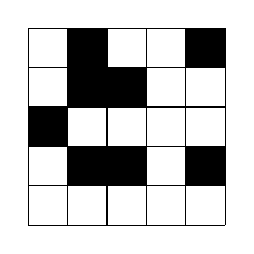
\begin{tikzpicture}[scale=0.5]
\fill[black] (1,1) rectangle (2,2);
\fill[black] (1,4) rectangle (2,5);
\fill[black] (4,1) rectangle (5,2);
\fill[black] (4,4) rectangle (5,5);
\fill[black] (1,3) rectangle (2,4);
\fill[black] (2,3) rectangle (3,4);
\fill[black] (2,1) rectangle (3,2);
\fill[black] (0,2) rectangle (1,3);
\draw (0,0) grid (5,5);
\end{tikzpicture}
\end{center}
contém duas dessas subgrades:
\begin{center}
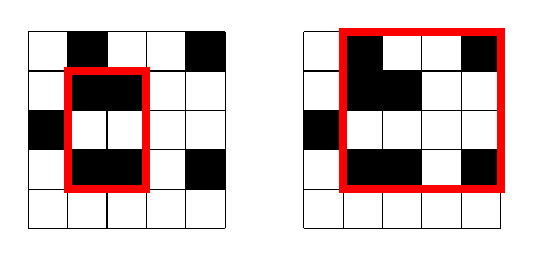
\begin{tikzpicture}[scale=0.5]
\fill[black] (1,1) rectangle (2,2);
\fill[black] (1,4) rectangle (2,5);
\fill[black] (4,1) rectangle (5,2);
\fill[black] (4,4) rectangle (5,5);
\fill[black] (1,3) rectangle (2,4);
\fill[black] (2,3) rectangle (3,4);
\fill[black] (2,1) rectangle (3,2);
\fill[black] (0,2) rectangle (1,3);
\draw (0,0) grid (5,5);

\fill[black] (7+1,1) rectangle (7+2,2);
\fill[black] (7+1,4) rectangle (7+2,5);
\fill[black] (7+4,1) rectangle (7+5,2);
\fill[black] (7+4,4) rectangle (7+5,5);
\fill[black] (7+1,3) rectangle (7+2,4);
\fill[black] (7+2,3) rectangle (7+3,4);
\fill[black] (7+2,1) rectangle (7+3,2);
\fill[black] (7+0,2) rectangle (7+1,3);
\draw (7+0,0) grid (7+5,5);

\draw[color=red,line width=1mm] (1,1) rectangle (3,4);
\draw[color=red,line width=1mm] (7+1,1) rectangle (7+5,5);
\end{tikzpicture}
\end{center}

Existe um algoritmo de tempo $O(n^3)$ para resolver o problema:
percorrer todos os $O(n^2)$ pares de linhas e para cada par
$(a,b)$ calcule o número de colunas que contêm um preto
quadrado em ambas as linhas em $O(n)$ tempo.
O código a seguir assume que $\texttt{color}[y][x]$
denota a cor na linha $y$ e coluna $x$:
\begin{lstlisting}
int count = 0;
for (int i = 0; i < n; i++) {
    if (color[a][i] == 1 && color[b][i] == 1) count++;
}
\end{lstlisting}
Então, essas colunas
contam para $\texttt{count}(\texttt{count}-1)/2$ subgrades com cantos pretos,
porque podemos escolher quaisquer dois deles para formar uma subgrade.

Para otimizar esse algoritmo, dividimos a grade em blocos
de colunas de forma que cada bloco consista em $N$
colunas consecutivas. Então, cada linha é armazenada como
uma lista de números de $N$ bits que descrevem as cores
dos quadrados. Agora podemos processar $N$ colunas ao mesmo tempo
usando operações de bits. No código a seguir,
$\texttt{color}[y][k]$ representa
um bloco de $N$ cores como bits.
\begin{lstlisting}
int count = 0;
for (int i = 0; i <= n/N; i++) {
    count += __builtin_popcount(color[a][i]&color[b][i]);
}
\end{lstlisting}
O algoritmo resultante funciona em $O(n^3/N)$ tempo.

Geramos uma grade aleatória de tamanho $2500 \times 2500$
e comparamos a implementação original e otimizada de bits.
Enquanto o código original levou 29,6 segundos,
a versão otimizada de bits levou apenas 3,1 segundos
com $N=32$ (números \texttt{int}) e 1,7 segundos
com $N=64$ (números \texttt{long long}).

\section{Programação dinâmica}

As operações de bits fornecem uma maneira eficiente e conveniente
de implementar algoritmos de programação dinâmica
cujos estados contêm subconjuntos de elementos,
porque esses estados podem ser armazenados como inteiros.
A seguir, discutimos exemplos de combinação
de operações de bits e programação dinâmica.

\subsubsection{Seleção ótima}

Como primeiro exemplo, considere o seguinte problema:
Somos dados os preços de $k$ produtos
ao longo de $n$ dias, e queremos comprar cada produto
exatamente uma vez.
No entanto, podemos comprar no máximo um produto
em um dia.
Qual é o preço total mínimo?
Por exemplo, considere o seguinte cenário ($k=3$ e $n=8$):
\begin{center}
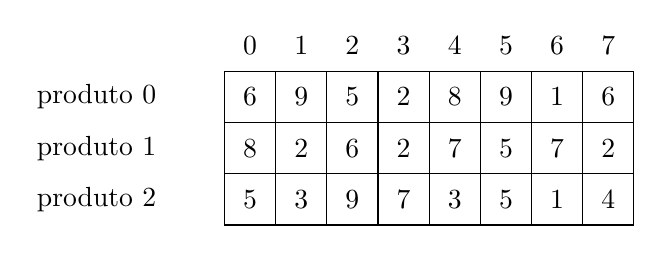
\begin{tikzpicture}[scale=.65]
    \draw (0, 0) grid (8,3);
    \node at (-2.5,2.5) {produto 0};
    \node at (-2.5,1.5) {produto 1};
    \node at (-2.5,0.5) {produto 2};

    \foreach \x in {0,...,7}
        {\node at (\x+0.5,3.5) {\x};}
    \foreach \x/\v in {0/6,1/9,2/5,3/2,4/8,5/9,6/1,7/6}
        {\node at (\x+0.5,2.5) {\v};}
    \foreach \x/\v in {0/8,1/2,2/6,3/2,4/7,5/5,6/7,7/2}
        {\node at (\x+0.5,1.5) {\v};}
    \foreach \x/\v in {0/5,1/3,2/9,3/7,4/3,5/5,6/1,7/4}
        {\node at (\x+0.5,0.5) {\v};}
\end{tikzpicture}
\end{center}
Neste cenário, o preço total mínimo é 5:
\begin{center}
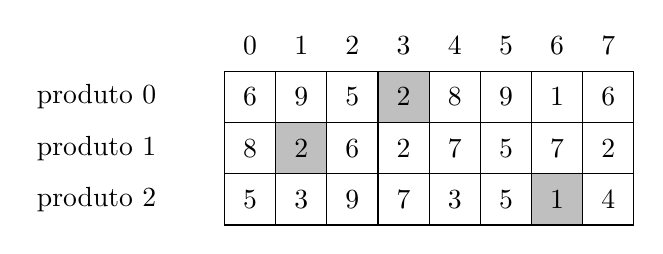
\begin{tikzpicture}[scale=.65]
    \fill [color=lightgray] (1, 1) rectangle (2, 2);
    \fill [color=lightgray] (3, 2) rectangle (4, 3);
    \fill [color=lightgray] (6, 0) rectangle (7, 1);
    \draw (0, 0) grid (8,3);
    \node at (-2.5,2.5) {produto 0};
    \node at (-2.5,1.5) {produto 1};
    \node at (-2.5,0.5) {produto 2};

    \foreach \x in {0,...,7}
        {\node at (\x+0.5,3.5) {\x};}
    \foreach \x/\v in {0/6,1/9,2/5,3/2,4/8,5/9,6/1,7/6}
        {\node at (\x+0.5,2.5) {\v};}
    \foreach \x/\v in {0/8,1/2,2/6,3/2,4/7,5/5,6/7,7/2}
        {\node at (\x+0.5,1.5) {\v};}
    \foreach \x/\v in {0/5,1/3,2/9,3/7,4/3,5/5,6/1,7/4}
        {\node at (\x+0.5,0.5) {\v};}
\end{tikzpicture}
\end{center}

Seja $\texttt{price}[x][d]$ o preço do produto $x$
no dia $d$.
Por exemplo, no cenário acima $\texttt{price}[2][3] = 7$.
Então, seja $\texttt{total}(S,d)$ o preço total mínimo
para comprar um subconjunto $S$ de produtos até o dia $d$.
Usando essa função, a solução para o problema é
$\texttt{total}(\{0 \ldots k-1\},n-1)$.

Primeiro, $\texttt{total}(\emptyset,d) = 0$,
porque não custa nada comprar um conjunto vazio,
e $\texttt{total}(\{x\},0) = \texttt{price}[x][0]$,
porque existe uma maneira de comprar um produto no primeiro dia.
Então, a seguinte recorrência pode ser usada:
\begin{equation*}
\begin{split}
\texttt{total}(S,d) = \min( & \texttt{total}(S,d-1), \\
& \min_{x \in S} (\texttt{total}(S \setminus x,d-1)+\texttt{price}[x][d]))
\end{split}
\end{equation*}
Isso significa que nós ou não compramos nenhum produto no dia $d$
ou compramos um produto $x$ que pertence a $S$.
Neste último caso, removemos $x$ de $S$ e adicionamos o
preço de $x$ ao preço total.

A próxima etapa é calcular os valores da função
usando programação dinâmica.
Para armazenar os valores da função, declaramos um array
\begin{lstlisting}
int total[1<<K][N];
\end{lstlisting}
onde $K$ e $N$ são constantes suficientemente grandes.
A primeira dimensão do array corresponde a uma
representação de bits de um subconjunto.

Primeiro, os casos onde $d=0$ podem ser processados da seguinte forma:
\begin{lstlisting}
for (int x = 0; x < k; x++) {
    total[1<<x][0] = price[x][0];
}
\end{lstlisting}
Então, a recorrência se traduz no seguinte código:
\begin{lstlisting}
for (int d = 1; d < n; d++) {
    for (int s = 0; s < (1<<k); s++) {
        total[s][d] = total[s][d-1];
        for (int x = 0; x < k; x++) {
            if (s&(1<<x)) {
                total[s][d] = min(total[s][d],
                                    total[s^(1<<x)][d-1]+price[x][d]);
            }
        }
    }
}
\end{lstlisting}
A complexidade de tempo do algoritmo é $O(n 2^k k)$.

\subsubsection{De permutações para subconjuntos}

Usando programação dinâmica, é frequentemente possível
transformar uma iteração sobre permutações em
uma iteração sobre subconjuntos\footnote{Essa técnica foi introduzida em 1962
por M. Held e R. M. Karp \cite{hel62}.}.
A vantagem disso é que
$n!$, o número de permutações,
é muito maior que $2^n$, o número de subconjuntos.
Por exemplo, se $n=20$, então
$n! \approx 2.4 \cdot 10^{18}$ e $2^n \approx 10^6$.
Assim, para certos valores de $n$,
podemos iterar eficientemente pelos subconjuntos, mas não pelas permutações.

Como exemplo, considere o seguinte problema:
Há um elevador com peso máximo $x$,
e $n$ pessoas com pesos conhecidos
que desejam ir do térreo
para o último andar.
Qual é o número mínimo de viagens necessárias
se as pessoas entrarem no elevador em uma ordem ótima?

Por exemplo, suponha que $x=10$, $n=5$
e os pesos são os seguintes:
\begin{center}
\begin{tabular}{ll}
pessoa & peso \\
\hline
0 & 2 \\
1 & 3 \\
2 & 3 \\
3 & 5 \\
4 & 6 \\
\end{tabular}
\end{center}
Nesse caso, o número mínimo de viagens é 2.
Uma ordem ótima é $\{0,2,3,1,4\}$,
que divide as pessoas em duas viagens:
primeiro $\{0,2,3\}$ (peso total 10),
e então $\{1,4\}$ (peso total 9).

O problema pode ser facilmente resolvido em $O(n! n)$ tempo
testando todas as possíveis permutações de $n$ pessoas.
No entanto, podemos usar programação dinâmica para obter
um algoritmo mais eficiente em tempo $O(2^n n)$.
A ideia é calcular para cada subconjunto de pessoas
dois valores: o número mínimo de viagens necessárias e
o peso mínimo das pessoas que viajam no último grupo.

Seja $\texttt{peso}[p]$ o peso da
pessoa $p$.
Definimos duas funções:
$\texttt{viagens}(S)$ é o número mínimo de
viagens para um subconjunto $S$,
e $\texttt{ultima}(S)$ é o peso mínimo
da última viagem.
Por exemplo, no cenário acima
\[ \texttt{viagens}(\{1,3,4\})=2 \hspace{10px} \textrm{e}
\hspace{10px} \texttt{ultima}(\{1,3,4\})=5,\]
porque as viagens ótimas são $\{1,4\}$ e $\{3\}$,
e a segunda viagem tem peso 5.
Claro, nosso objetivo final é calcular o valor
de $\texttt{viagens}(\{0 \ldots n-1\})$.

Podemos calcular os valores
das funções recursivamente e então aplicar
programação dinâmica.
A ideia é percorrer todas as pessoas
que pertencem a $S$ e escolher de forma ótima
a última pessoa $p$ que entra no elevador.
Cada escolha desse tipo gera um subproblema
para um subconjunto menor de pessoas.
Se $\texttt{ultima}(S \setminus p)+\texttt{peso}[p] \le x$,
podemos adicionar $p$ à última viagem.
Caso contrário, precisamos reservar uma nova viagem
que inicialmente contém apenas $p$.

Para implementar a programação dinâmica,
declaramos um array
\begin{lstlisting}
pair<int,int> melhor[1<<N];
\end{lstlisting}
que contém para cada subconjunto $S$
um par $(\texttt{viagens}(S),\texttt{ultima}(S))$.
Definimos o valor para um grupo vazio da seguinte forma:
\begin{lstlisting}
melhor[0] = {1,0};
\end{lstlisting}
Então, podemos preencher o array da seguinte forma:

\begin{lstlisting}
for (int s = 1; s < (1<<n); s++) {
    // valor inicial: n+1 viagens sao necessarias
    melhor[s] = {n+1,0};
    for (int p = 0; p < n; p++) {
        if (s&(1<<p)) {
            auto opcao = melhor[s^(1<<p)];
            if (opcao.second+peso[p] <= x) {
                // adicionar p a uma viagem existente
                opcao.second += peso[p];
            } else {
                // reservar uma nova viagem para p
                opcao.first++;
                opcao.second = peso[p];
            }
            melhor[s] = min(melhor[s], opcao);
        }
    }
}
\end{lstlisting}
Observe que o loop acima garante que
para quaisquer dois subconjuntos $S_1$ e $S_2$
tais que $S_1 \subset S_2$, processamos $S_1$ antes de $S_2$.
Assim, os valores de programação dinâmica são calculados na
ordem correta.

\subsubsection{Contando subconjuntos}

Nosso último problema neste capítulo é o seguinte:
Seja $X=\{0 \ldots n-1\}$, e cada subconjunto $S \subset X$
recebe um inteiro $\texttt{valor}[S]$.
Nossa tarefa é calcular para cada $S$
\[\texttt{soma}(S) = \sum_{A \subset S} \texttt{valor}[A],\]
ou seja, a soma dos valores dos subconjuntos de $S$.

Por exemplo, suponha que $n=3$ e os valores são os seguintes:
\begin{multicols}{2}
\begin{itemize}
\item $\texttt{valor}[\emptyset] = 3$
\item $\texttt{valor}[\{0\}] = 1$
\item $\texttt{valor}[\{1\}] = 4$
\item $\texttt{valor}[\{0,1\}] = 5$
\item $\texttt{valor}[\{2\}] = 5$
\item $\texttt{valor}[\{0,2\}] = 1$
\item $\texttt{valor}[\{1,2\}] = 3$
\item $\texttt{valor}[\{0,1,2\}] = 3$
\end{itemize}
\end{multicols}
Nesse caso, por exemplo,`'
\begin{equation*}
\begin{split}
\texttt{soma}(\{0,2\}) &= \texttt{valor}[\emptyset]+\texttt{valor}[\{0\}]+\texttt{valor}[\{2\}]+\texttt{valor}[\{0,2\}] \\ 
                      &= 3 + 1 + 5 + 1 = 10.
\end{split}
\end{equation*}

Como há um total de $2^n$ subconjuntos,
uma possível solução é percorrer todos
os pares de subconjuntos em tempo $O(2^{2n})$.
No entanto, usando programação dinâmica, podemos
resolver o problema em tempo $O(2^n n)$.
A ideia é focar em somas onde os
elementos que podem ser removidos de $S$ são restritos.

Seja $\texttt{parcial}(S,k)$ a soma dos
valores dos subconjuntos de $S$ com a restrição
de que apenas os elementos $0 \ldots k$
podem ser removidos de $S$.
Por exemplo,
\[\texttt{parcial}(\{0,2\},1)=\texttt{valor}[\{2\}]+\texttt{valor}[\{0,2\}],\]
porque podemos remover apenas os elementos $0 \ldots 1$.
Podemos calcular os valores de \texttt{soma} usando
os valores de \texttt{parcial}, porque
\[\texttt{soma}(S) = \texttt{parcial}(S,n-1).\]
Os casos base para a função são
\[\texttt{parcial}(S,-1)=\texttt{valor}[S],\]
porque nesse caso nenhum elemento pode ser removido de $S$.
Então, no caso geral, podemos usar a seguinte recorrência:
\begin{equation*}
    \texttt{parcial}(S,k) = \begin{cases}
               \texttt{parcial}(S,k-1) & k \notin S \\
               \texttt{parcial}(S,k-1) + \texttt{parcial}(S \setminus \{k\},k-1) & k \in S
           \end{cases}
\end{equation*}
Aqui focamos no elemento $k$.
Se $k \in S$, temos duas opções: podemos manter $k$ em $S$
ou removê-lo de $S$.

Há uma maneira particularmente inteligente de implementar o
cálculo das somas. Podemos declarar um array
\begin{lstlisting}
int soma[1<<N];
\end{lstlisting}
que conterá a soma de cada subconjunto.
O array é inicializado da seguinte forma:
\begin{lstlisting}
for (int s = 0; s < (1<<n); s++) {
    soma[s] = valor[s];
}
\end{lstlisting}
Então, podemos preencher o array da seguinte forma:
\begin{lstlisting}
for (int k = 0; k < n; k++) {
    for (int s = 0; s < (1<<n); s++) {
        if (s&(1<<k)) soma[s] += soma[s^(1<<k)];
    }
}
\end{lstlisting}
Esse código calcula os valores de $\texttt{parcial}(S,k)$
para $k=0 \ldots n-1$ no array \texttt{soma}.
Como $\texttt{parcial}(S,k)$ é sempre baseado em
$\texttt{parcial}(S,k-1)$, podemos reutilizar o array
\texttt{soma}, o que gera uma implementação muito eficiente.

